\begin{figure}[t] \centering 
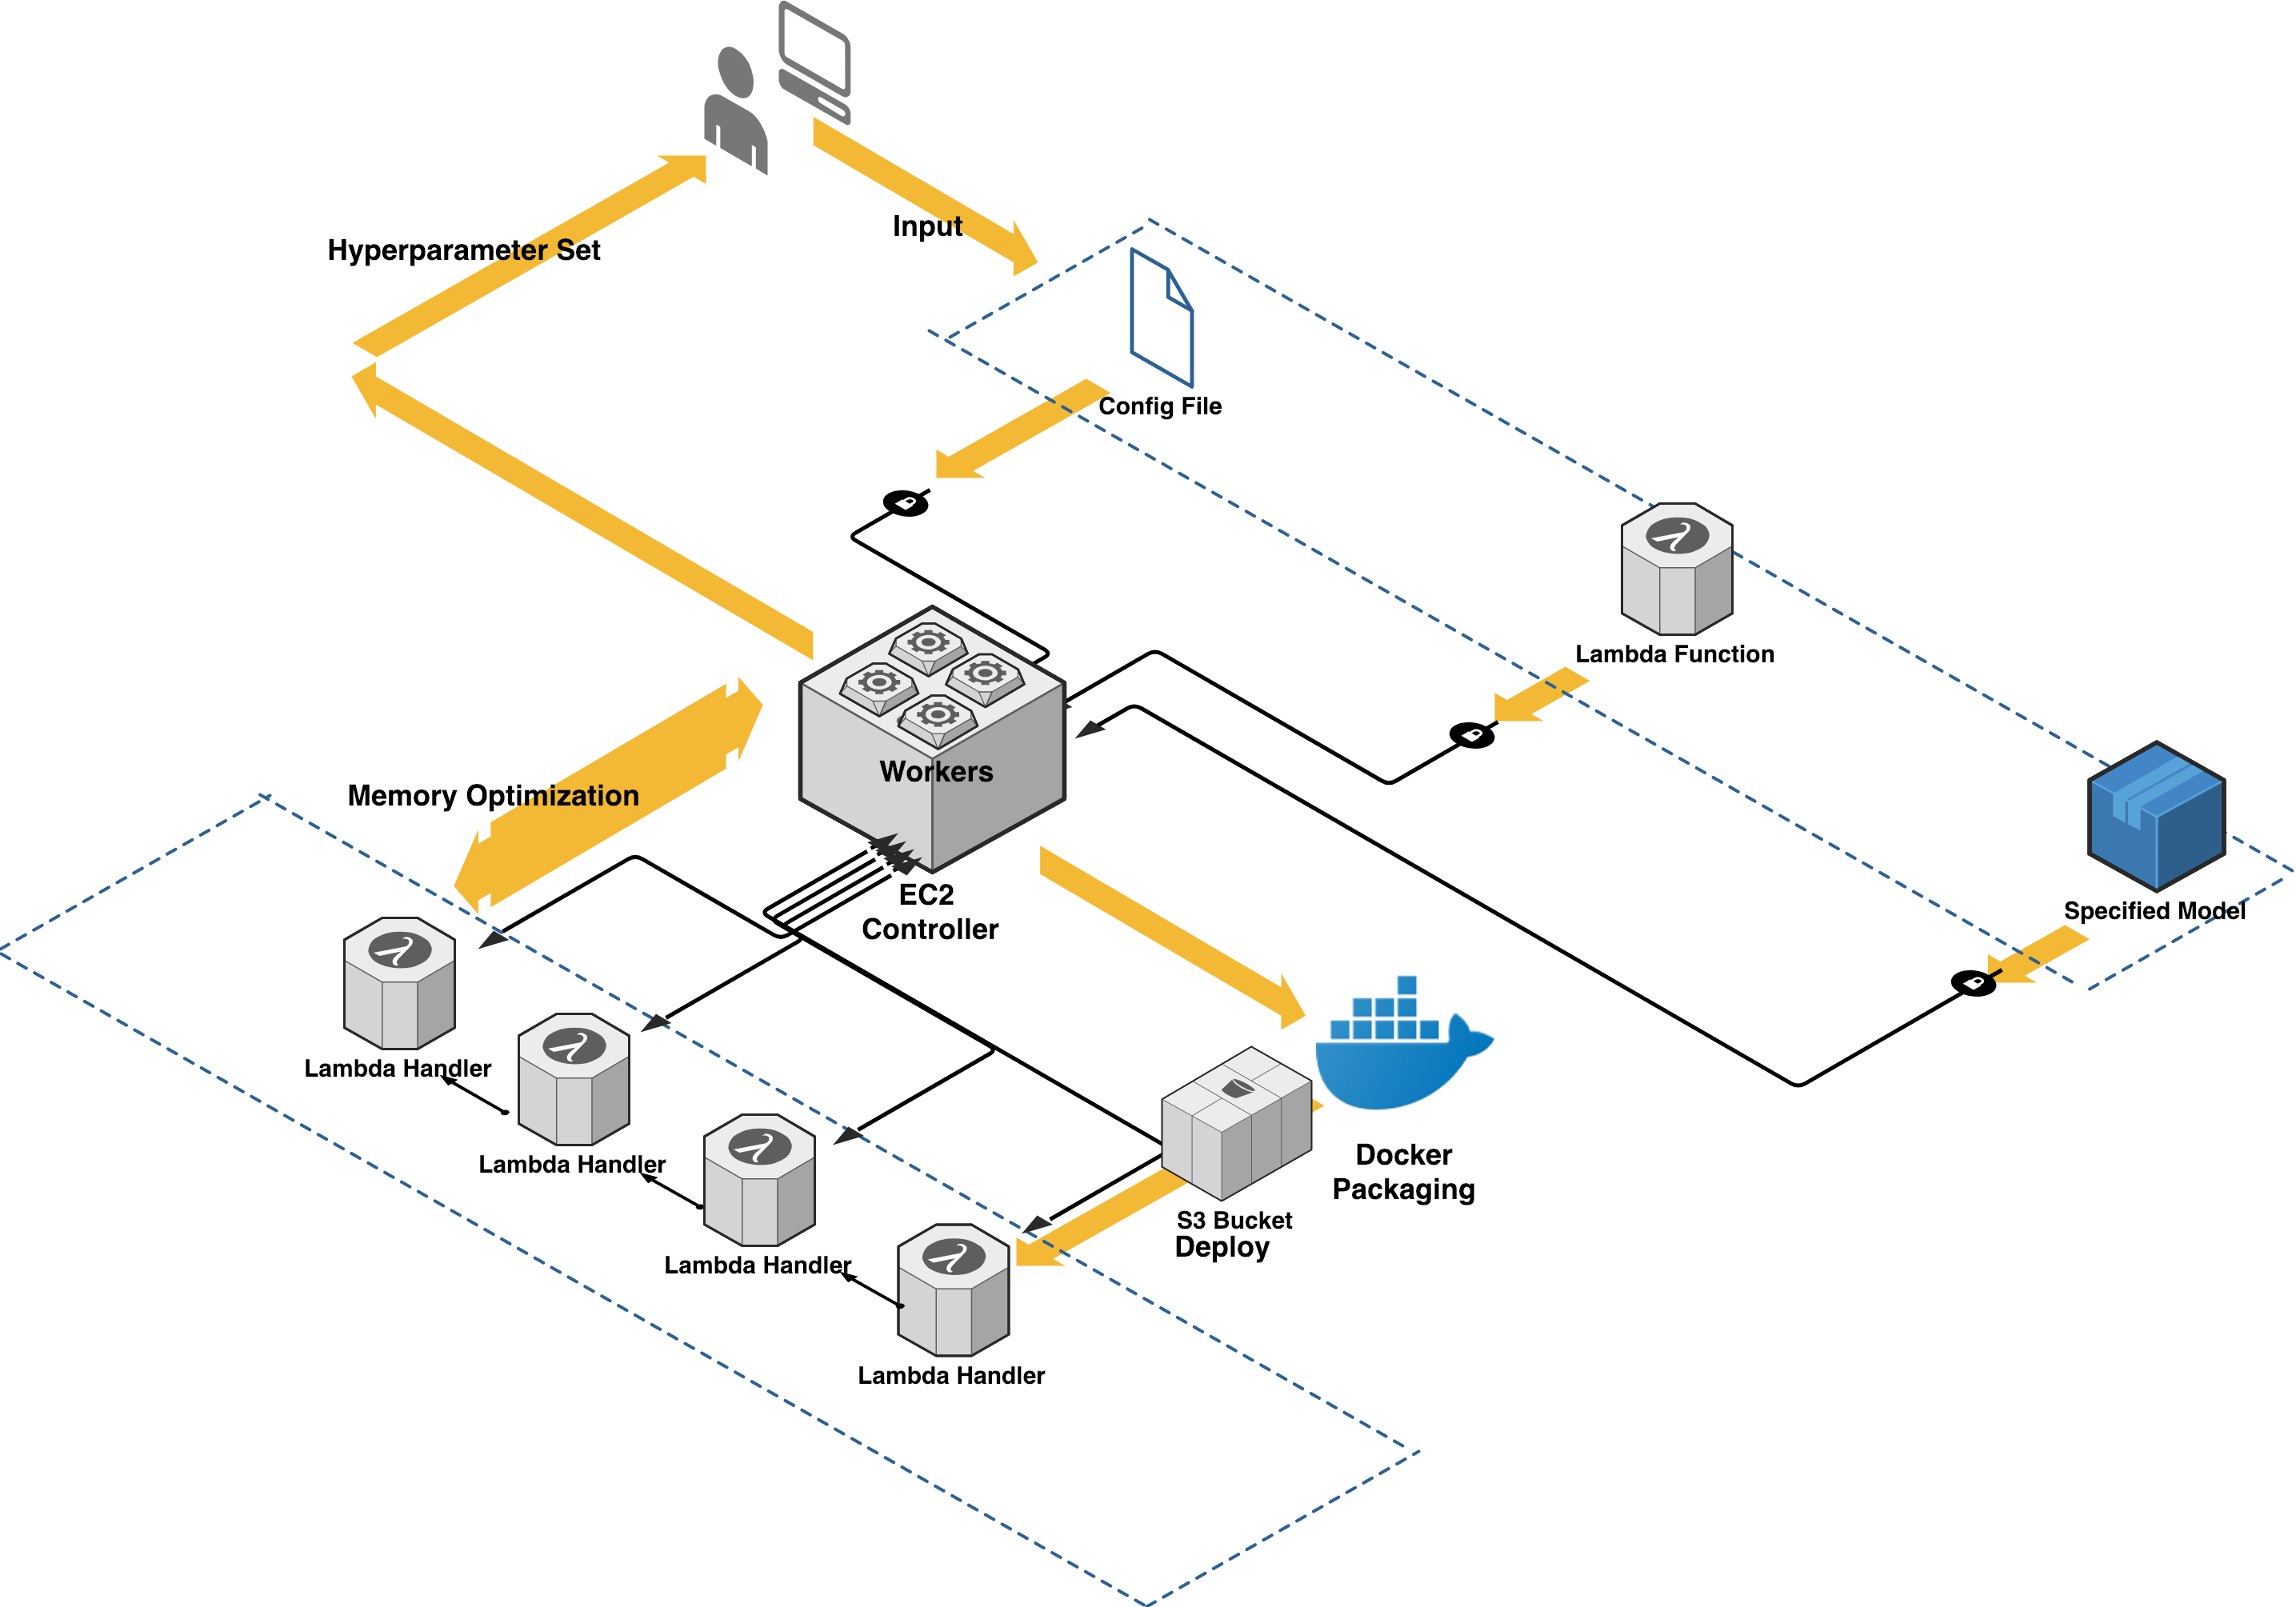
\includegraphics[scale=0.08]{Seneca}
\caption{The architecture of Seneca. 
User specifies hyperparameter options in the configuration file and provides lambda function. Seneca automatically package, deploy and optimize lambda function on AWS before completing grid search process and selecting best hyperparameter setting.
\label{fig:seneca}}
% \vspace{-0.2in}
\end{figure}

To facilitate model optimization on serverless architecture, we have developed Seneca, a framework of  hyperparameter tuning for machine learning algorithm on AWS Lambda. The automated Seneca pipeline consists of packaging, deployment, serverless function optimization and hyperparameter tuning. Figure~\ref{fig:seneca} portrays the architecture of Seneca: the upper right front are three inputs from users: configuration file, specified model, and lambda function. Configuration file is where users specify all hyperparameter options and used by Seneca to create search space. Specified model is the implementation library of training and testing for certain machine learning model and provides clearly defined methods. Lambda function is the function handler that executes on AWS lambda. It downloads the dataset from S3 bucket, splits it by desired training and testing ratio, trains the specified model and returns the testing score. 

\subsection{Packaging and Deployment}

After receiving these three inputs, Seneca launches a docker container that simulates the runtime of AWS Lambda. The container will compress the lambda function with all required libraries from specified model in a zip package and upload to S3 bucket. Using S3 bucket as an intermediate storage is to avoid the size limitation (10MB) of deployment package directly transported to AWS Lambda. Once uploaded to S3 bucket, docker container will deploy the deployment package to AWS lambda by AWS Command line Interface~\cite{ref:awscli} for Lambda. 


\subsection{Allocated memory optimization}

Seneca has a component of optimizer that allows user to optimize allocated memory of lambda function. The mechanism of optimizer is based on our hypothesis of disproportional increase of computational power bound to allocated memory of lambda function. In other words, additional computational power brought by extra allocated memory reduces the billed duration and possibly overall cost as well. Seneca optimizer tries to find this "sweet-spot" of allocated memory leading to lowest compute charge.

Instead of exhaustively searching for all 46 possible memory configurations of lambda function, we designed a heuristic that complete the task faster and more economically. The detailed heuristic is outlined in the Algorithm~\ref{algo:optimizer}. Seneca optimizer first probes function by a user-defined payload to obtain the memory used by function as start point. It also defines two double-end queues (deque) to store a certain number (N) of historical allocated memory and compute charge data. While the current allocated memory is less than or equal to 3008 MB, optimizer keeps probing function and calculated compute charge by current allocated memory and billed duration. Two exit conditions are established in the heuristic: first, compute charge monotonically increases in the whole length of deque; second, the increase slope is greater than a threshold. Once optimizer find both conditions hold, it will pop the left-most value from allocated memory deque and configure the lambda function at such memory. After repetitive experiments, we find the setting of N = 5 and slope = 1 has the highest possibility to find the lowest compute charge.

\begin{algorithm}[]
\SetAlgoLined
\KwData{Typical payload}
\KwResult{Optimal allocated memory}
Find memory used by payload as start point\;
Define deques for struct of allocated memory \& compute charge\;
 \While{allocated memory $\leq$ 3008 MB}{
  
  \eIf{compute charge monotonically increase in deque \& slope $\geq$ 1}{
   Popleft from deque\;
   Configure allocated memory of function\; 
   Exit\;
   }{
   Increase allocated memory by 64 MB\;
   Probe lambda function\;
   Append new struct to deque\;
  }
 }
 \caption{Seneca Optimizer Heuristic}
 \label{algo:optimizer}
\end{algorithm}

\subsection{Tuning process}

In order to invoke lambda function concurrently, Seneca integrates with Celery~\cite{ref:celery}. Celery is an asynchronous task queue based on distributed message passing. Celery workers are working processes that pick up tasks from the queue, execute tasks and store the asynchronous result at backend (Redis~\cite{ref:redis} in our case). Based on user-defined configuration file, Seneca creates a list of payloads that contains values of hyperparameters and the whole list covers the entire Cartesian product search space. Every payload launches a Celery task, on which a worker executes by triggering lambda function and insert a new record of the returned evaluation score and corresponding hyperparameter setting to backend database. 

After the comprehensive searching, Seneca will extract all records within search space and select the best result. Up to users' specification, Seneca returns either hyperparameter setting or a serialized model trained by this setting.